\documentclass[a4paper,twocolumn,english,fontsize=7,DIV=16]{scrartcl}

% Localization options
\usepackage[english]{babel}
\usepackage{blindtext}
\usepackage[T1]{fontenc}
\usepackage[utf8]{inputenc}

% Enhanced verbatim sections. We're mainly interested in
% \verbatiminput though.
\usepackage{verbatim}

% PDF-compatible landscape mode.
% Makes PDF viewers show the page rotated by 90°.
\usepackage{pdflscape}

% Advanced tables
\usepackage{tabu}
\usepackage{longtable}
\usepackage{dcolumn}
\newcolumntype{d}[1]{D{.}{\cdot}{#1} }

% Fancy tablerules
\usepackage{booktabs}

% Graphics
\usepackage{graphicx}

% Current time
\usepackage[useregional=numeric]{datetime2}

% Float barriers.
% Automatically add a FloatBarrier to each \section
\usepackage[section]{placeins}

% Custom header and footer
\usepackage{fancyhdr}

\usepackage{layout}

% Math tools
\usepackage{mathtools}
% Math symbols
\usepackage{amsmath,amsfonts,amssymb}
\usepackage{amsthm}

% SI units
\usepackage{siunitx}
\DeclareSIUnit\Molar{\textsc{m}}
\DeclareSIUnit\mole{mol}
\DeclareSIUnit\rpm{rpm}
\DeclareSIUnit\cfu{cfu}

% Chemistry
\usepackage{mhchem}

% Subfigures & captions
\usepackage{subcaption}
\usepackage{wrapfig}

\DeclarePairedDelimiter\abs{\lvert}{\rvert}

\pagestyle{plain}
% \fancyhf{}
% \lhead{}
% \lfoot{}
% \rfoot{}
% 
% Source code & highlighting
\usepackage{listings}

% Convenience commands
\newcommand{\mailsubject}{1611 - Biochemie 1}
\newcommand{\maillink}[1]{\href{mailto:#1?subject=\mailsubject}
                               {#1}}

% Should use this command wherever the print date is mentioned.
\newcommand{\printdate}{\today}

\subject{1611 - Biochemie 1}

\title{Summary}

\author{Michael Senn \maillink{michael.senn@students.unibe.ch} - 16-126-880}

\date{\printdate}

% Needs to be the last command in the preamble, for one reason or
% another. 
\usepackage{hyperref}


\begin{document}
\maketitle

\section{Moleküle des Lebens}

\begin{description}
	\item[Leben] Weit weg von chem. Gleichgewicht da zB Produkte System
		verlassen, Selbstreplikation mit Fehlermöglichkeit (=
		Evolution). Braucht Energie.
	\item[Künstliches Leben] Botom Up (Erschaffung aus nichts) vs Top down
		(Reduzierung existierendes Lebens)
	\item[Domänen d Lebens]: Eukaryonten, Bakterien, Archaen
	\item[LUCA] Last universal common ancestor of life
	\item[Katalyse] Senkung der Aktivierungsenergie, kein Einfluss auf
		$\Delta G$.
	\item[Reaktionsbeschleunigung] Beschleunigung der Reaktion durch
		Temperatur (Stabilität Biomoleküle), Konzentration Edukte
		(Preis), Kopplung an schnelle Reaktion, Katalyse.
	\item[Pathways] Metabolisch: Produziert Energie oder natürliche
		Materialien. Signaltransduktion: Leitet Informationen weiter.
	\item[RNA Welt] DNA hat keine katalytische Aktivität und komplexe
		Replikation, also Entstehen des Lebens aus RNA Enzymen (zb
		Ribosom).
\end{description}

\subsection{Energie \& Kohlenstoffquellen}

\begin{figure}[h]
	\centering
	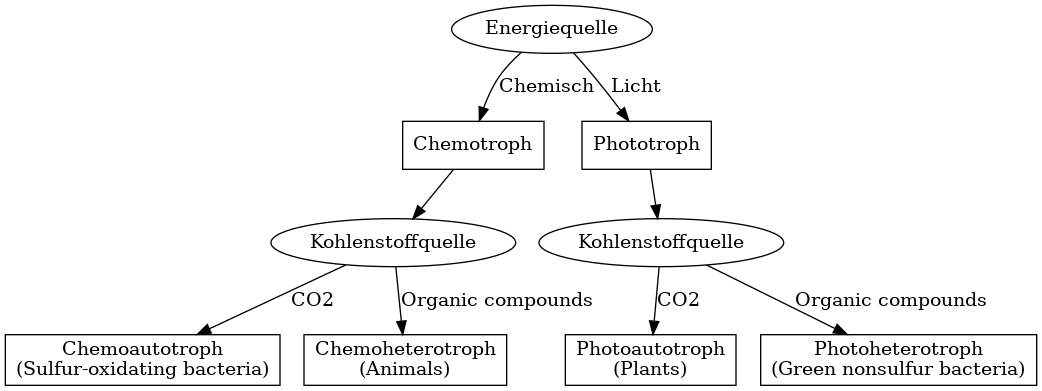
\includegraphics[width=\linewidth]{graphs/ec_quellen.png}
	\caption{Classification based on carbon and energy source}
\end{figure}

\subsection{Bakterienzellen}

\begin{description}
	\item[Pili] Adhesion to other cells
	\item[Nucleoid] Long circular DNA molecule
	\item[Cell envelope] encompasses cell
	\item[Cytoplasma] \SIrange{300}{500}{\milli\Molar} proteins
	\item[Flagella] Movement
\end{description}

\subsubsection{Komponenten}

\begin{tabu}{lll}
	\toprule
	Struktur & Aufbau & Funktion \\
	\midrule
	Zellwand & Peptidoglycan & Mechanischer Support \\
	Zellmembran & Lipide \& Proteine & Permeabilitäts-Schranke \\
	Nucleoid & DNA \& Proteine & Genetische Information \\
	Ribosome & RNA \& Proteine & Protein-Synthese \\
	Pili / Flagellen & Proteine & Adhäsion / Fortbewegung \\
	Zytoplasma & Wässrige Lösung & Ort des Metabolismus \\
	\bottomrule
\end{tabu}

\subsubsection{Gram-positiv / negativ}

Bezeichnet ob Zelle einfärbbar mit Gention-Violett. Negative Organismen haben
äussere Membran und Peptidoglycan-Schicht, Positive keine äussere Membran dafür
eine dickere Peptidoglycanschicht.

\subsubsection{Archaen}

Archaen (!= Bakterien) haben keine äussere Membran, und eine
Pseudopeptidoglycanschicht. Ether statt Ester in Zellwand für
Kopfgruppe-Glycerol Verbindung. Stabiler gegen Hydrolyse. Verzweigte
Phytonyl-Gruppen machen Membran rigide und undurchdringbar für zB Salze.

\subsubsection{Funktionelle Gruppen}

\begin{figure}[h]
	\centering
	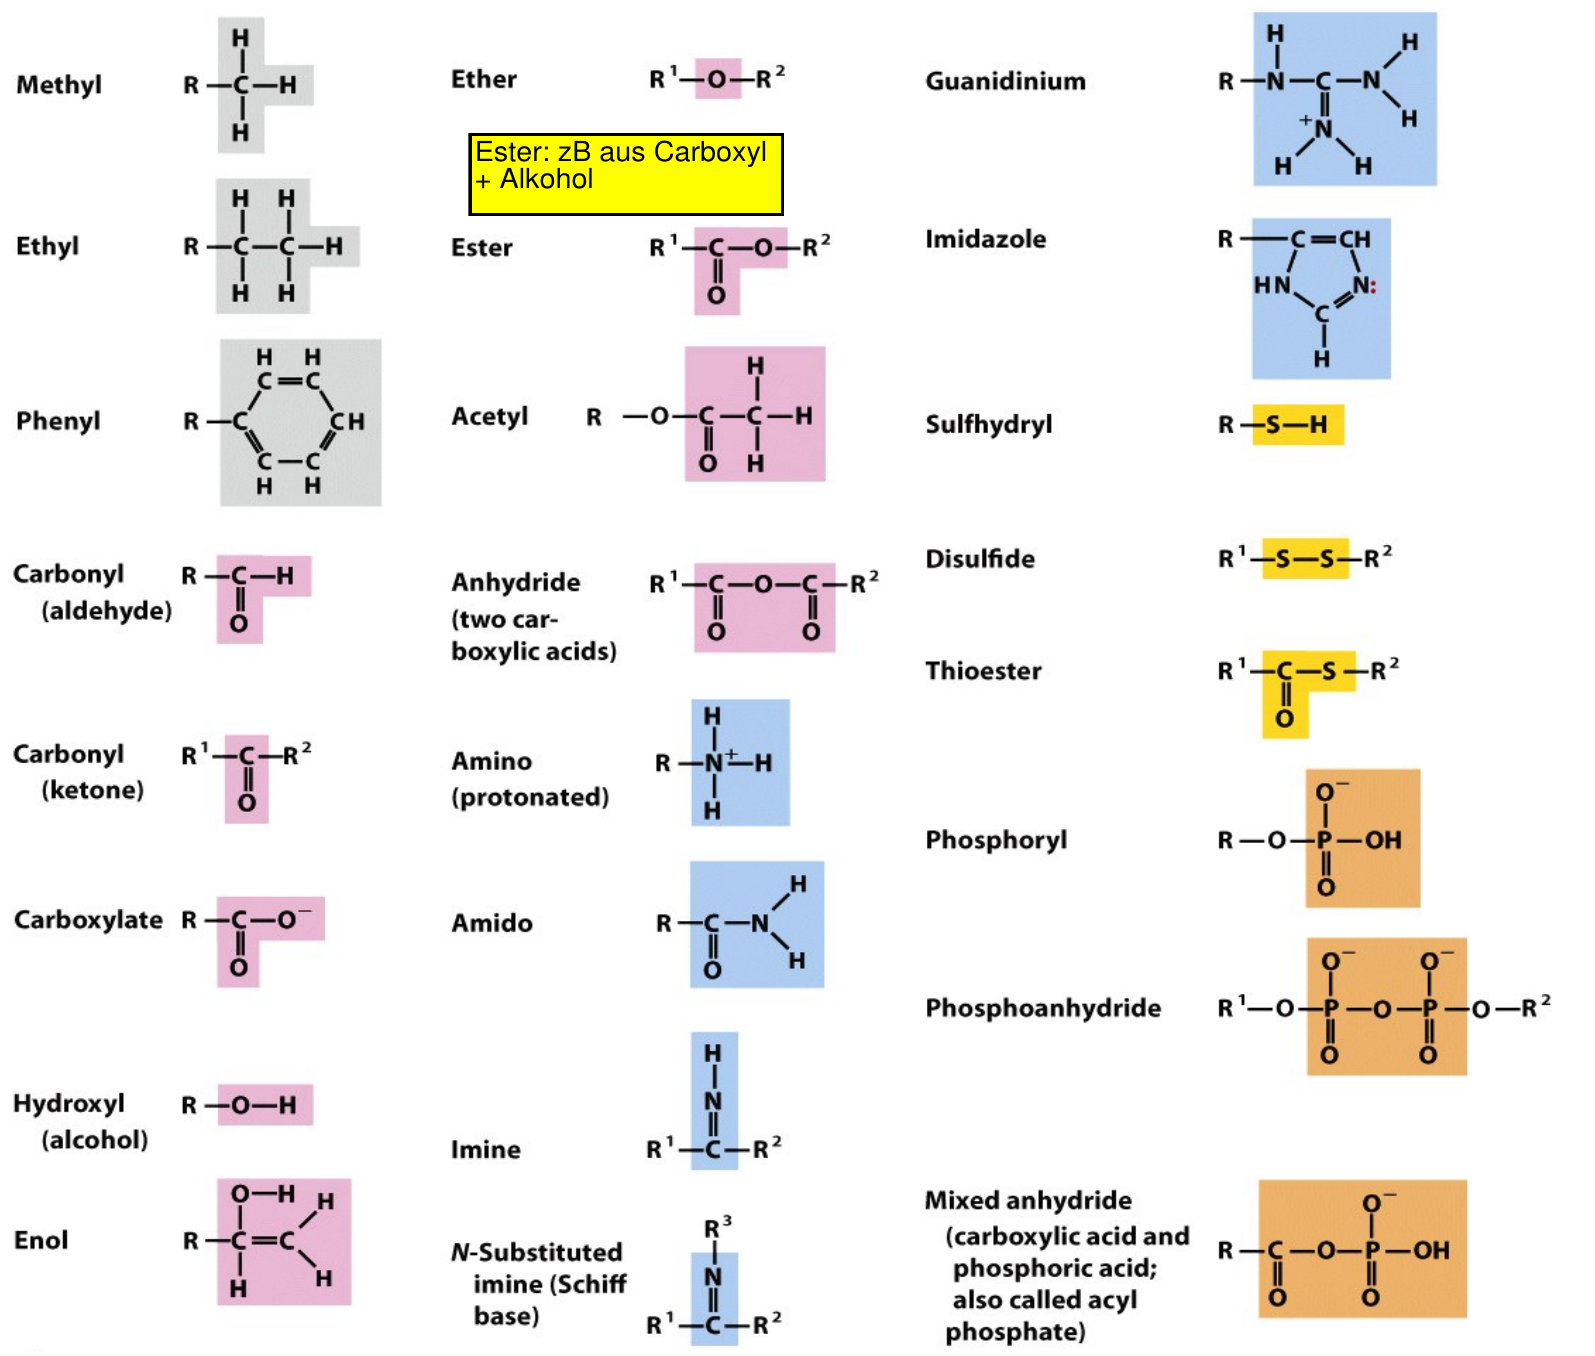
\includegraphics[width=\linewidth]{img/funktionale_gruppen.png}
	\caption{Funktionelle Gruppen}
\end{figure}

\subsubsection{Isomerie}

\begin{figure}[h]
	\centering
	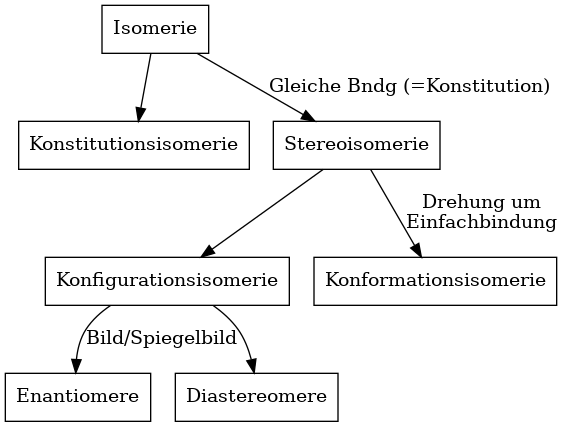
\includegraphics[width=\linewidth]{graphs/isomerie.png}
	\caption{Isomerie}
\end{figure}

\begin{description}
	\item[Enantiomere] Gleiche physikalische \& chemische Eigenschaften
		(exkl Polarisierung von Licht), unterschiedliche biologische
		Eigenschaften. Gemisch zweier Enantiomere = Racemat.
	\item[Diastereomer] zB cis/trans, Unterschiedliche physikalische \&
		chemische Eigenschaften.
\end{description}

\subsection{Gibbs Energie}

$\Delta G = \Delta H - T \Delta S$, $\Delta H$ = Enthalpie
(endotherm/exotherm), $\Delta S$ = Entropie. \SI{0}{\kelvin} =
\SI{-237.15}{\celsius}. $\Delta G < 0 \Rightarrow$ spontan.

\section{Wasser}

\begin{description}
	\item[H-Brücke] Nicht-kovalete Bndg, 3-4 je \ce{H2O} Molekül wenn
		flüssig. Moleküle in oberster Schicht nach unten gezogen -
		Oberflächenspannung.
	\item[Wechselwirkungen] Ionisch: zwischen Ionen oder Ion/Dipol. Dipol:
		Zwischen ungeladenen aber polaren Molekülen. VdW: Unabhängig
		von Polarität. Hydrophober Effekt: Unpolare Moleküle in Wasser,
		Entropie-bedingt.
	\item[Hydrophober Effekt] Wasser-Käfig um apolare Moleküle entspricht
		Ordnung. Micellenbildung verringert Anzahl Moleküle in Käfig,
		entropisch begünstigt. Ebenso zB Begünstigung Enzym-Substrat
		Bindung falls Bindungsstelle hydrophob.
	\item[Gebundenes Wasser] Wasser in Protein ohne osmotische Aktivität
		(keine Diffusion), zB spezifische Funktion in Protein. Bsp
		Cytochrom F: Elektronentransport (Proton Hopping)
	\item[Gleichgewichtskonstante] $A \Rightarrow B + C$, $K_{eq} =
		\frac{[B] \cdot [C]}{[A]}$
\end{description}

\subsection{Schwache Säuren}

$p_{ka}$: PH bei dem \SI{50}{\percent} dissoziert. Henderson-Hasselbalch:
$\text{pH} = p_{ka} + \log\left(\frac{[A-]}{[HA]}\right)$. Puffer am effektivsten bei
$\text{pH} = p_{ka} \pm 1$.

\section{Aminosäuren / Peptide}

\begin{figure}
	\centering
	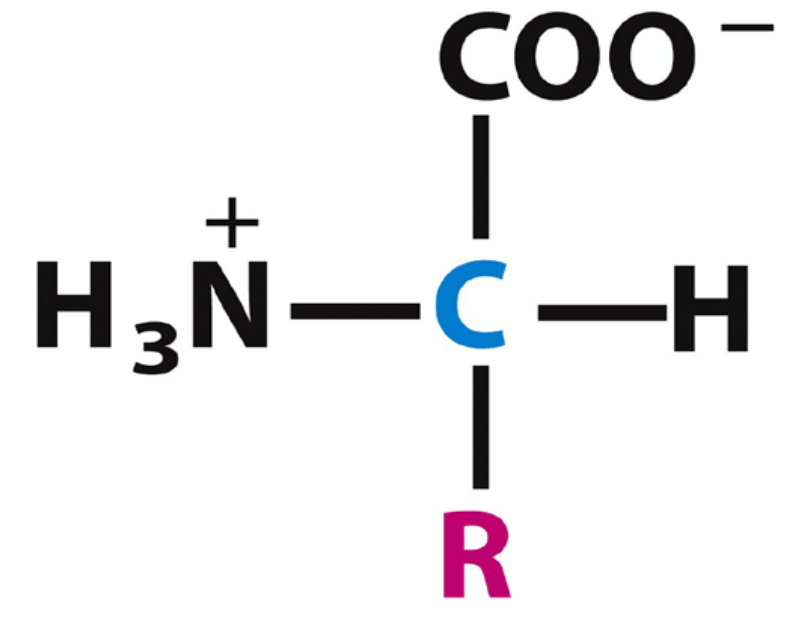
\includegraphics[width=\linewidth]{img/as.png}
	\caption{Allgemeine Struktur}
\end{figure}

\begin{figure}
	\centering
	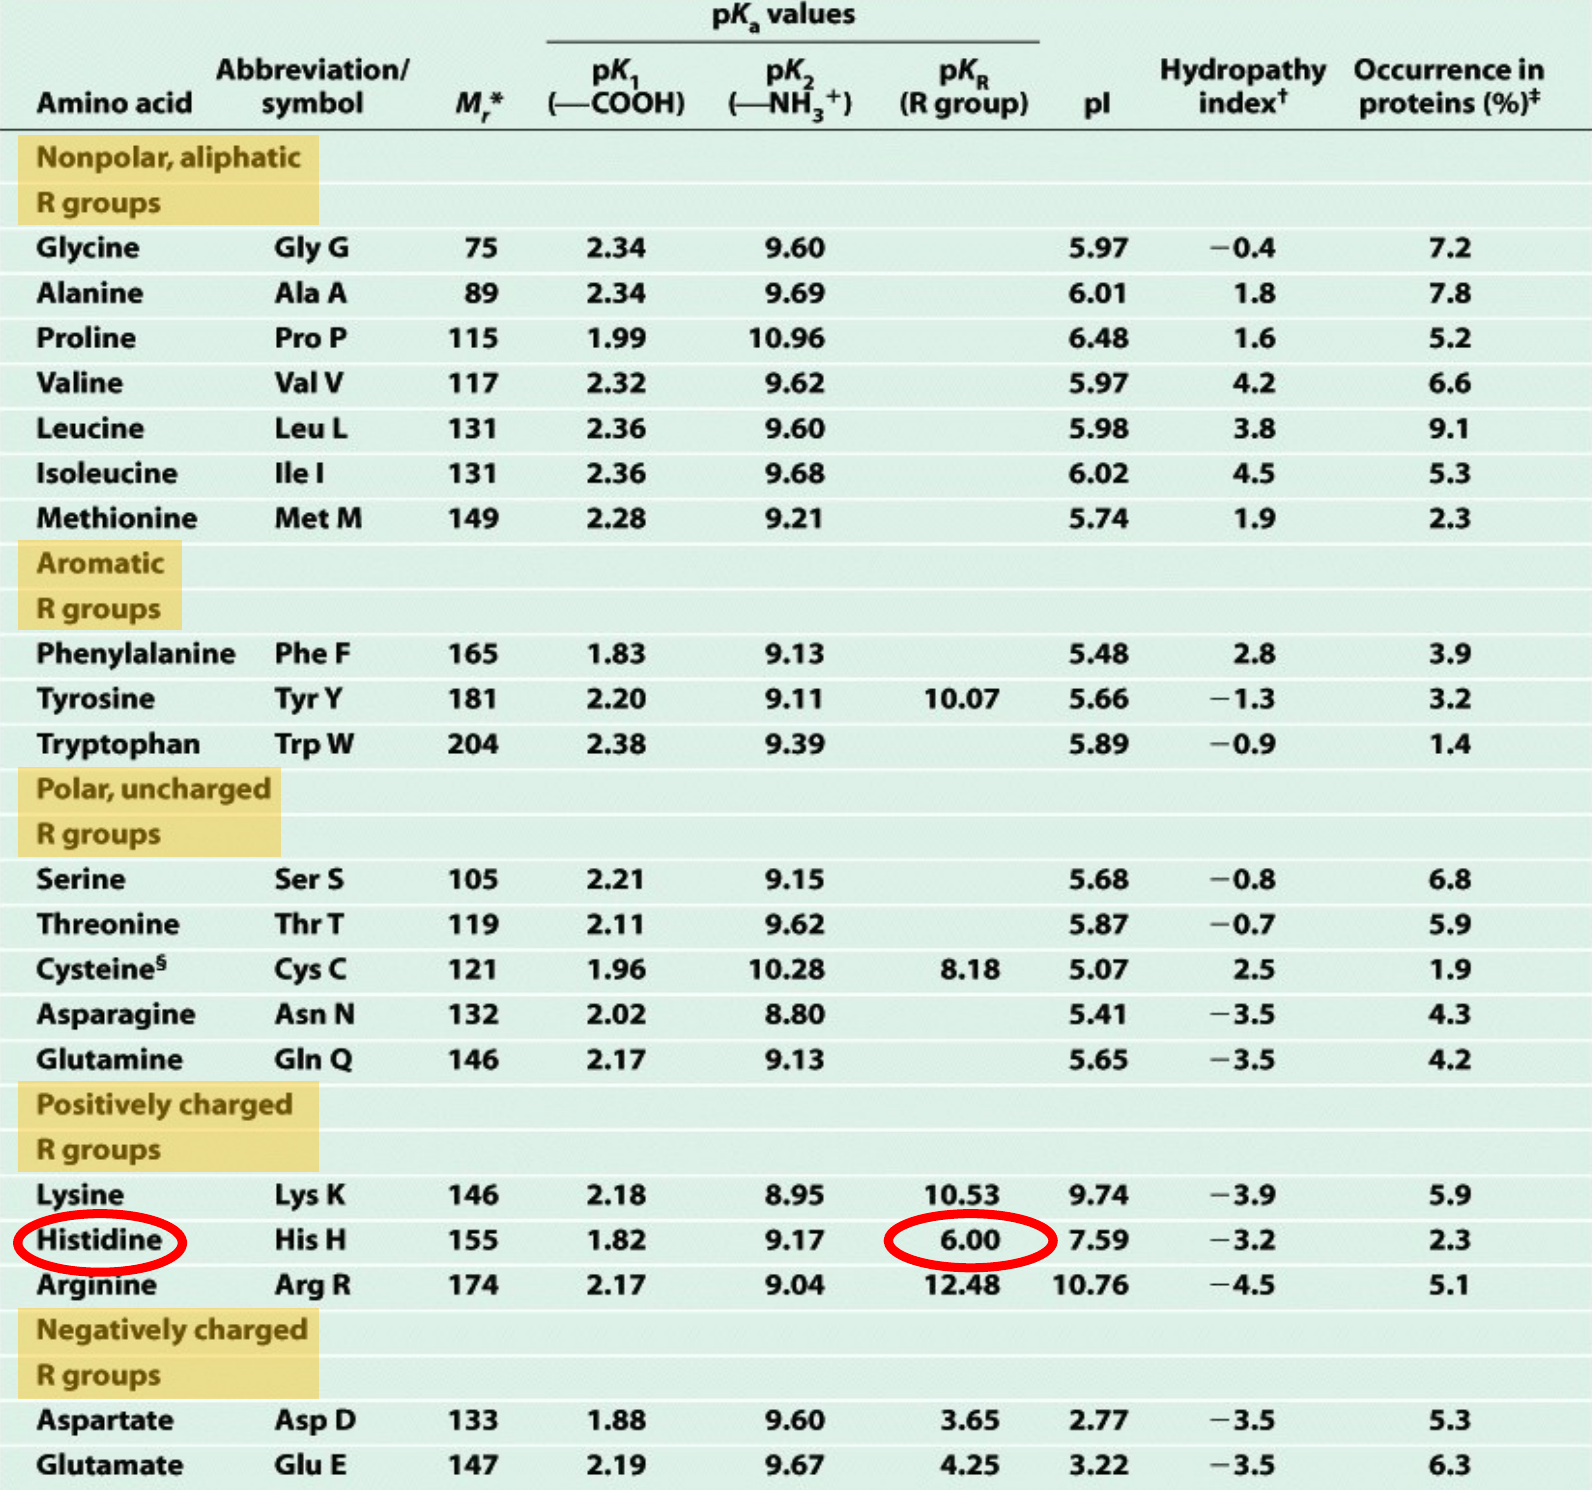
\includegraphics[width=\linewidth]{img/as_liste.png}
	\caption{Liste der AS}
\end{figure}

\begin{description}
	\item [Nomenklatur AS] In Biochemie ab $\alpha$-C Atom, welches Amino und Carbonsäure tragt.
	\item[Fischer Projektion] Stärkst oxidiertes Atom nach oben. Vertikal =
		In Ebene rein, Horizontal = Aus Ebene raus. Falls Rest mit
		höchster Priorität nach Rechts dann R, sonst L.  Priorität:
		COOH > COH > CH2OH > CH3 > H.
	\item[Aromatischer Rest] Absorption bei \SIrange{270}{280}{\nm}
	\item[Ionisierung von AS] Bei saurem pH Carboxyl und Amino protoniert,
		bei neutralem nur Amino protoniert, bei basischem beide
		deprotoniert. Einfluss auf Ladung (Positiv/Neutral/Negativ).
		Auch für Rest relevant.
	\item[$p_{ka}$ Werte] Amino in neutraler Umgebung (\ce{CH3}) 10.6, bei
		AS (Nähe \ce{O}) 9.6. Carbonsäure neutral 4.8, in AS (pos.
		Ladung \ce{NH3+}) 2.3.
	\item[Isoelektrischer Punkt $p_I$] Durchschnitt der zwei $p_{ka}$ am
		nächsten an erwartetem $p_I$.
	\item [Peptide] Kondenstationsprodukte von AS. Nummerierung ab
		Amino-terminalem Ende. Stabile Verbindung, Spaltung chemisch
		(\ce{HCl} kochend) oder Enzyme, zB Trypsin (nach positiv
		geladener AS) oder Chymotrypisi (nach aromatischer AS). Freie
		Enden \& Seitenketten können ionisieren, charakteristischen
		$p_I$.
	\item[Proteine] Polypeptide mit Kofaktoren (non-AS funktionelle
		Komponenten, entweder Coenzyme (nicht-kovalent) oder
		Prosthetische Gruppen (oft kovalent)), oder sonstigen
		Modifikationen.
	\item[Aktivität] \si{U} = \si{\micro \mole \text{ Substrat} \per \min} at \SI{25}{\celsius}
	\item[Spezifische Aktivität] \si{U \per \mg \text{ Proteingemisch}}
	\item[Chromatographie] Auftrennung nach Ladung / Grösse / Affinität
	\item[Elektrophorese] Auftrennung nach Grösse \& Konformation (SDS
		Page: Denaturierend, nur nach Grösse)
	\item[Disulfidbrücken] Aufbrechen durch Oxidation/Reduktion (zB DTT)
	\item[Homologe Sequenzen] Gemeinsame evolutionäre Abstammung.
	\item[Konvergenz]: Sequenz ähnlich weil selber oder ähnliche Funktion, aber unabhängige Evolution.
	\item[Ortholog / Paralog]: Ortholog: Homolog in verschiedenen Spezies
		wegen gemeinsamen Vorfahren, Paralog: Homolog wegen
		Genduplikation innerhalb Genom.
\end{description}

\begin{figure}
	\centering
	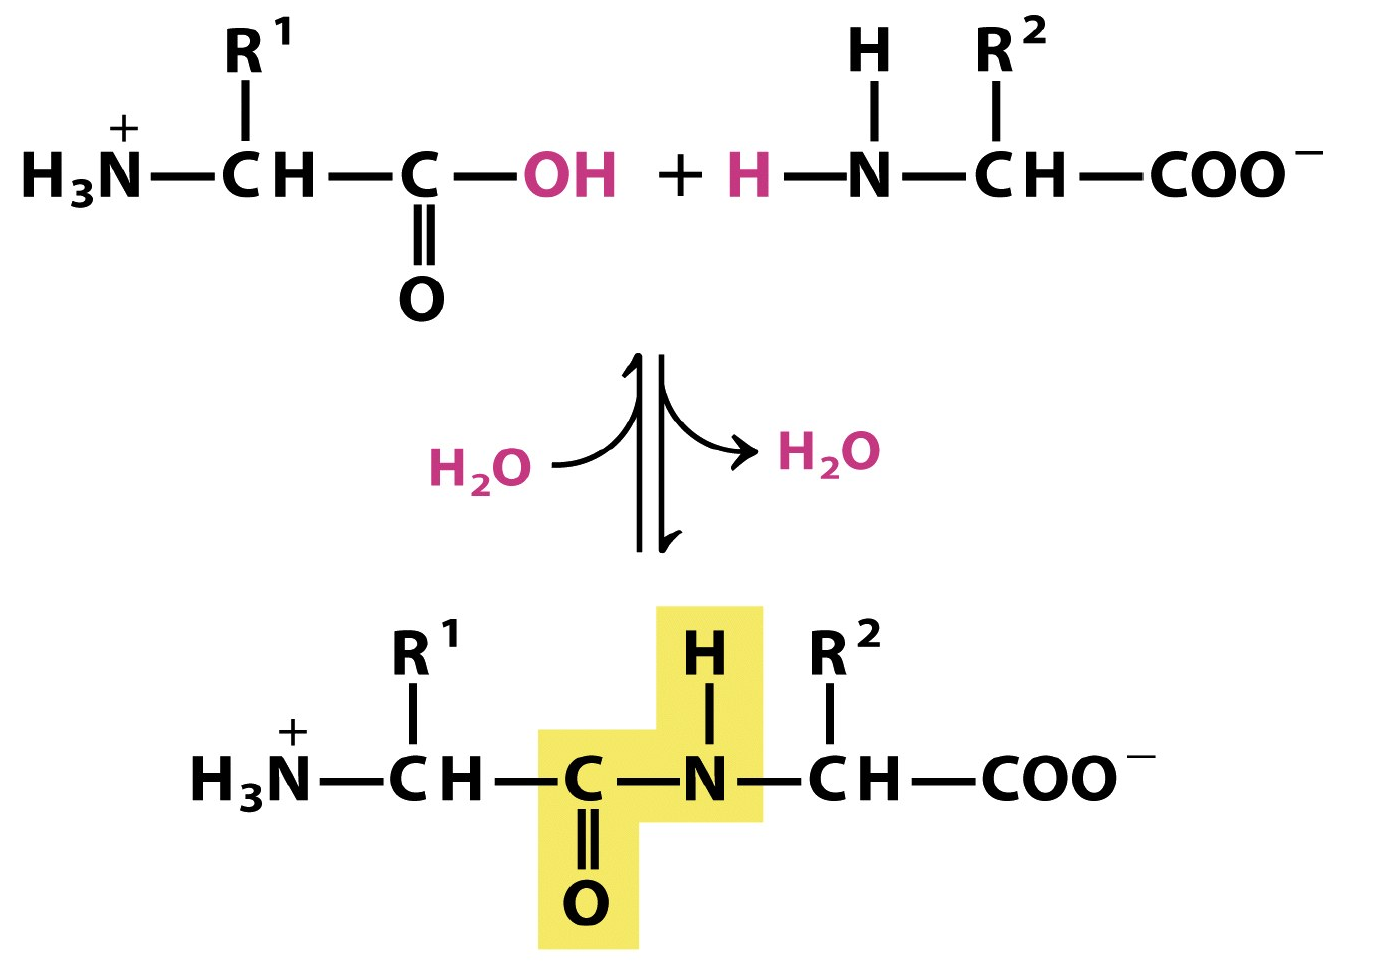
\includegraphics[width=\linewidth]{img/peptid_kond.png}
	\caption{Peptid Kondensation}
\end{figure}

\section{Proteinstruktur}

Ungefaltenes Protein hat hohe konformationelle Entropie, aber nicht kovalente
\& kovalente Wechselwirkungen stabilisieren Faltungsintermediate nd Endprodukt.
Hydrophobe Wechselwirkungen essentiell für erste Schritte.

\begin{description}
	\item[Peptidbindung] Starr, fast immer so dass \ce{H} trans zu \ce{O}
		der Carbonylgruppe aufgrund Dipol. Drehung um $\alpha$-C aber
		möglich, damit Wechselwirkungen zwischen Seitenketten.
	\item[Erkennung Faltung] Helices, Faltblätter, ... Häufig optisch
		aktiv. Antikörper. Verhalten in (non-SDS) Gelelektrophorese.
	\item[$\alpha$-Helix]: H-Brücken zwischen nahen (Sequenz) Einheiten.
		Jeweils AS 1/8, 2/9, ... übereinander. Seitenketten senkrecht
		auf Achse. Kleine hydrophoben AS gut für Helix. Prolin zerstört
		Struktur da keine Rotation möglich, Gly da Konformation
		ungünstigt. Rechtsgängig.
	\item[$\beta$-Faltblatt] H-Brücken zwischen räumlich nahen Sequenzen.
		Seitenketten abwechselnd oben/unten aus Blatt.
		Parallel/antiparalle. Anti stabiler da H-Brücken gerader.
	\item[$\beta$-Turns] \SI{180}{\degree} Richtungsänderung aus 4 AS, 2/3
		häufig Prolin da "gerne" in cis Konformation (\SI{6}{\percent}
		cis).
	\item[Tertiärstruktur] Fibrilläre Protein meist unlöslich, aus 2D
		Strukturen aufgebaut (zB Kollagen). Globuläre \ce{H2O}-\&
		lipdid-löslich (zB Myoglobin). Kollagen aus linksgängigen
		Ketten, drei zu rechtsgängiger Helix stabilisiert via
		H-Brücken, viele davon zu Fibrille.
	\item[Domäne] Teil der Polypeptidkette der sich autonom faltet oder
		relativ zu Rest des Proteins bewegen kann.
	\item[Denaturierung] Verlust der Struktur und Aktivität aufgrund Hitze,
		pH, organische Lösungsmittel (Interaktion mit hydrophobem Teil
		des Proteins), chaotrophe Stoffe (da Zerstörung H-Brücken im
		Wasser, damit Wegfall des hydrophoben Effekts)
	\item[Chaperone / Chaperonine] Chaperone verhindern falsche Faltungen
		durch Verhindern der Aggregation ungefaltener Protein, binden
		an hydrophobe Bereiche. Chaperonine fördern Faltung aktiv
		("Behälter für Faltung) unter Energieverbrauch.
\end{description}

\section{Protein-Liganden Interaktion}

\begin{description}
	\item[Ligand] Bindet nicht-kovalent an Bindungsstelle des Proteins.
		$k_a$ = Assoziationsgeschwindigkeit, $k_d$ =
		Dissoziationsgeschwindigkeit.  $K_a = \frac{k_a}{k_d}$ =
		Ggw-Konstante der Bindung (Assoziationskonstante), $K_d =
		K_a^{-1}$. $\Theta = \frac{[PL]}{[PL] + [P]} = \frac{[L]}{[L] +
		K_d}$. $K_d = P_{50}$ Liganden-Konzentration bei der $\Theta =
		0.5$.
	\item[Induced fit] Konformationsänderung nach Liganden-Bindung.
	\item[2,3-Biphosphoglycerat] Stabilisiert T-Zustand von Hb, dh senkt
		Bindungsaffinität der Hb - O Bindung. Mehr 2,3... -> Weniger
		starke Bindung, höhere $K_d$
	\item[Hämoglobin] Bindent \ce{O2} via Häm in Proteintasche, verhindert
		Oxidation von \ce{Fe2+} zu \ce{Fe3+}, senkt Affinität von Häm
		zu \ce{CO} (nur 200 statt 20k so stark).
	\item[Positive Kooperativität] Erste Liganden-Bindung erhöht Affinität
		für zweite, zB Hämoglobin. Führt zu sigmoider Kurve des
		$\Theta$ zu $[L]$ Graphen. Auch durch \ce{CO} ausgelöst,
		verhindert Abgabe in Gewebe.
	\item[Bohr Effekt] pH Unterschied Lunge / Gewebe (Lunge 0.2 basischer)
		fördert Bindung von \ce{O2} in Lunge, Abgabe in Gewebe.
	\item[\ce{CO2} Transport] \SI{75}{\percent} als Teil des
		Kohlensäure-Bicarbonat Buffersystems als \ce{HCO3-} + H+ in
		Blut. \SI{25}{\percent}  n Form von Carbamat an N-Terminalem
		Ende von Hb.
\end{description}

\section{Enzyme}

\begin{description}
	\item[Enzym] Katalytisch aktives Makromolekül, oft globuläre Proteine,
		teils auch RNAs. Umsetzung Substrat in aktivem Zentrum.
		Erniedrigung Aktivierungsenergie. Erhöhen
		Reaktionsgeschwindigkeit um $10^5$ bis $10^17$ durch günstige
		Positionierung, Stabilisierung T-State.
	\item[Reaktionsgeschwindigkeit] Erster Ordnung (ein Substrat) $V =
		k[S]$, zweiter Ordnung $V = k [S_1][S_2]$. $\Delta G^\circ = -R
		T \log(K_{eq})$, $R = \SI{8.314}{\J \per \mol}$
	\item[Katalysearten] S/B (Protonierung zwecks erreichen T-State),
		kovalent (Zwischenprodukt, A-B + X -> A-X + B -> A + B + X),
		Metallionen (zB Redox), elektrostatisch (Wechselwirkungen mit
		T-State).
	\item[Ribosom-katalysierte Reaktionen] Gleiche Mechanismen wie
		Protein-Enzyme, $10^5$ bis $10^11$ Erhöhung. Häufig fest
		gebundenes Wasser.
	\item[Michaelis] Mit E+S <-> ES <-> E + P, $k_1$ V der ersten Hin-,
		$k_{-1}$ der entsprechenden Rückreaktion: $K_m = \frac{k_2 +
		k_{-1}}{k_1}$ Substratkonzentration bei der $V = 0.5 V_{max}$.
		$V_0 = \frac{V_{max} [S]}{k_m + [S]} = \frac{k_2[E][S]}{K_m +
		[S]}$
	\item[Reaktionsintermediate] zB ES, EP Komplexe. Stabile Intermediate
		einer Reaktion.
	\item[Übergangszustände / T-State] Bei A -> B, Zwischenzustand zwischen
		A und B, sehr kurzlebig.
\end{description}

\begin{figure}
	\centering
	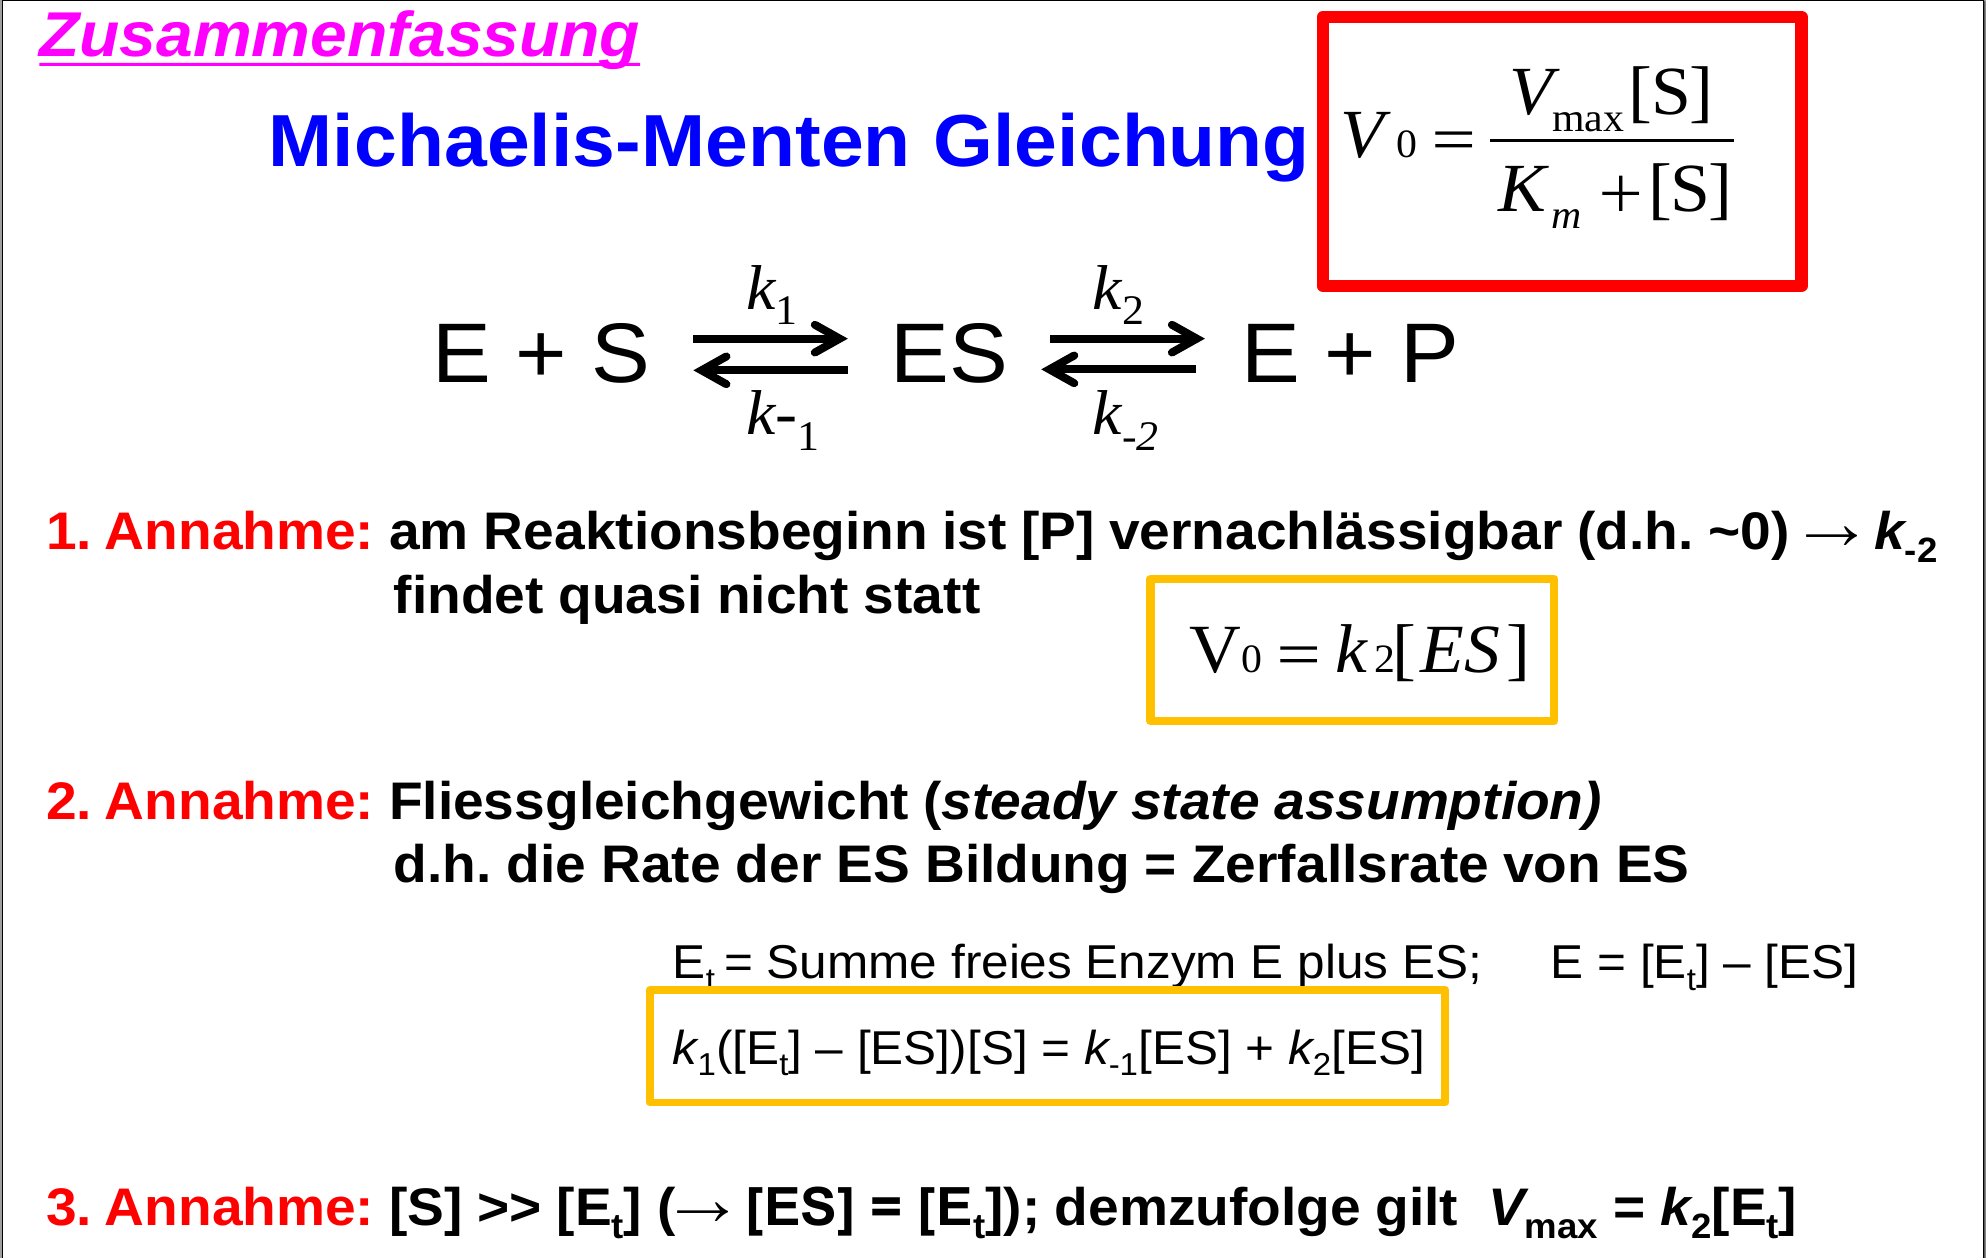
\includegraphics[width=\linewidth]{img/michaelis.png}
	\caption{Michaelis-Menten Gleichung}
\end{figure}

\begin{figure}
	\centering
	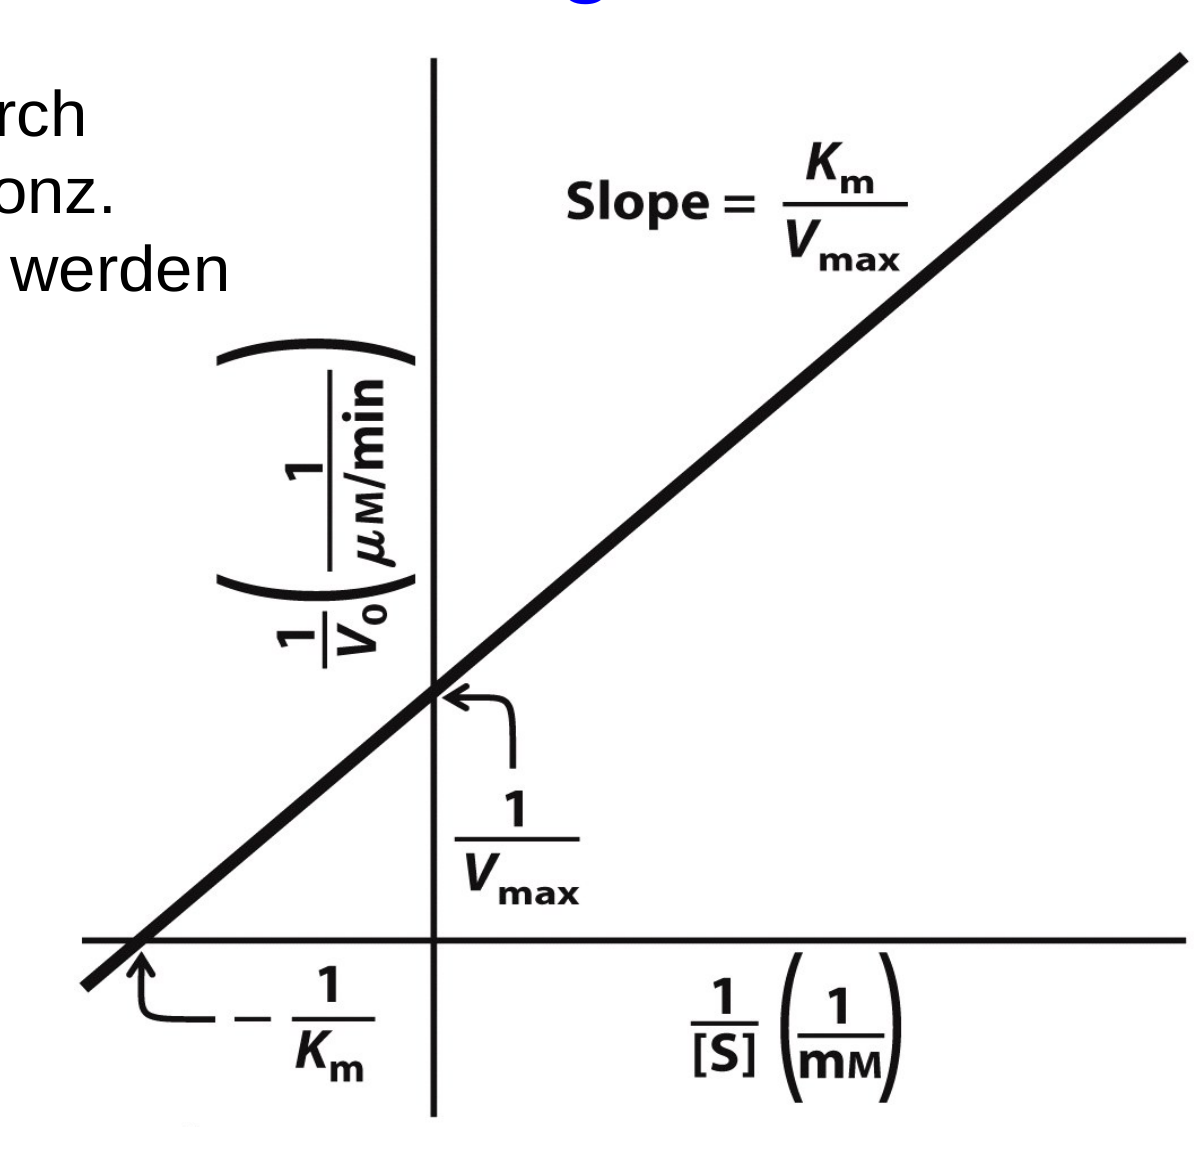
\includegraphics[width=\linewidth]{img/lb.png}
	\caption{Lineweaver-Burke Plot}
\end{figure}

\subsection{Inhibition}

\begin{description}
	\item[Irreversibel] Reagiert mit Enzym, permanente Inaktivierung.
		Toxisch. zB Ricin.
	\item[Reversibel] Bindet und dissoziiert rasch an und von Enzym. zB
		strukturelle Analogen zu Substrat, bindet an freies Enzym, oder
		E-S Komplexe. Kompetitiv: Bindet an gleiche Stelle wie
		Substrat. $V_{max}$ bleibt gleich, Steigung in LB Plot steigt
		mit Inhibitor-Konzentration. Nicht-kompetitiv: $V_max$ und
		$K_m$ verändern sich.
\end{description}

\section{Kohlenhydrate}

\begin{description}
	\item[Kohlenhydrate] Meist \ce{C_n(H2O)_n}. Energiequelle \& Speicher,
		Strukturelle Komponente, Informations-Molekül.
	\item[Epimere] Diastereomere die sich bei 1 C-Atom unterscheiden.
	\item[Halbacetale / Halbketale] Ringstruktur ab 5 C-Atomen, Alkohol zu
		Aldehyd/Keton Ringschluss. Acetale/Ketale sobald resultierender
		Alkohol weiteren Ringschluss eingeht. Gleichgewicht zwischen
		Ketten- und Ring-Form der Zucker. Aldehyde in Ketten sind
		reduktiv, erlaubt Detektion.
	\item[Glykosidische Bindung] Bindung zwischen Disacchariden via 2
		Hydroxygruppen, Abgang Wasser.
	\item[Nomenklatur] $C_1$ = neben O, trägt Alkohol.
	\item[Glycogen] $\alpha$1-4 Verknüpfte, $\alpha$1-6 verzweigte
		Glucosen. Hauptspeicher in Tieren.
	\item[Stärke] $\alpha$1-4 unverzweigte Ketten (Amylose), $\alpha$1-6
		Verzweigungen alle 24-30 Einheiten (Amylopectin). Hauptspeicher
		in Pflanzen.
	\item[Polysaccharide] Viele non-reduzierenden Enden, gleichzeitiger Abbau.
	\item[Zellulose] Unverzweigtes Homopolysaccharid von Glucose,
		$\beta$1-4 Ketten stabilisiert mit H-Brücken. $\beta$1-4 von
		Tieren nicht hydrolisierbar.
	\item[Glycoproteine] Protein + Oligosaccharid, dient Protein/Protein
		Erkennung in zB Immunsystem.
	\item[Glycolipide] Membranbestandteil von Tieren \& Pflanzen.
\end{description}

\begin{figure}
	\centering
	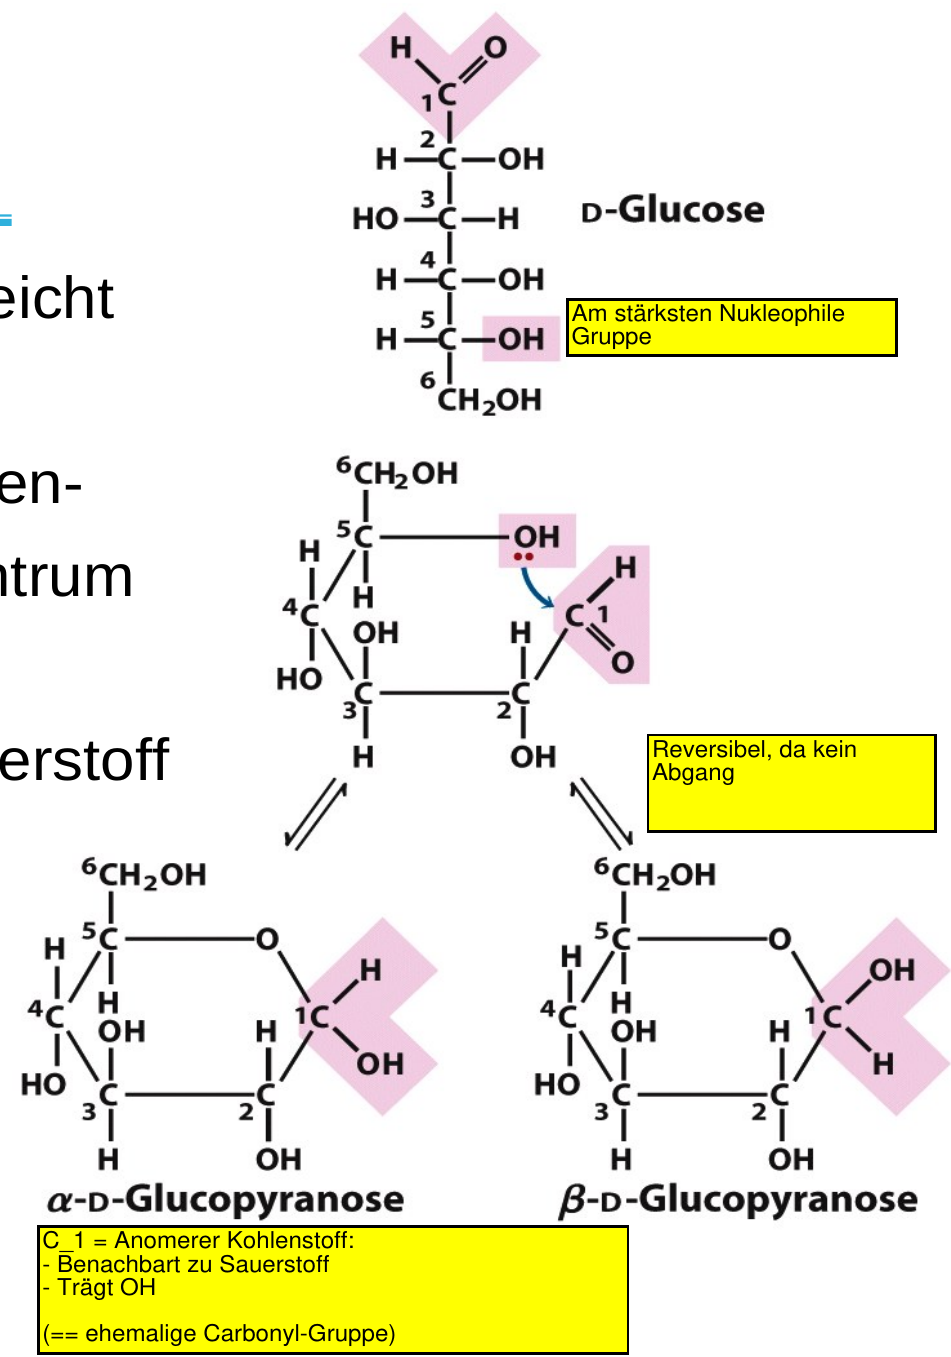
\includegraphics[width=\linewidth]{img/glucose.png}
	\caption{Glucose}
\end{figure}

\begin{figure}
	\centering
	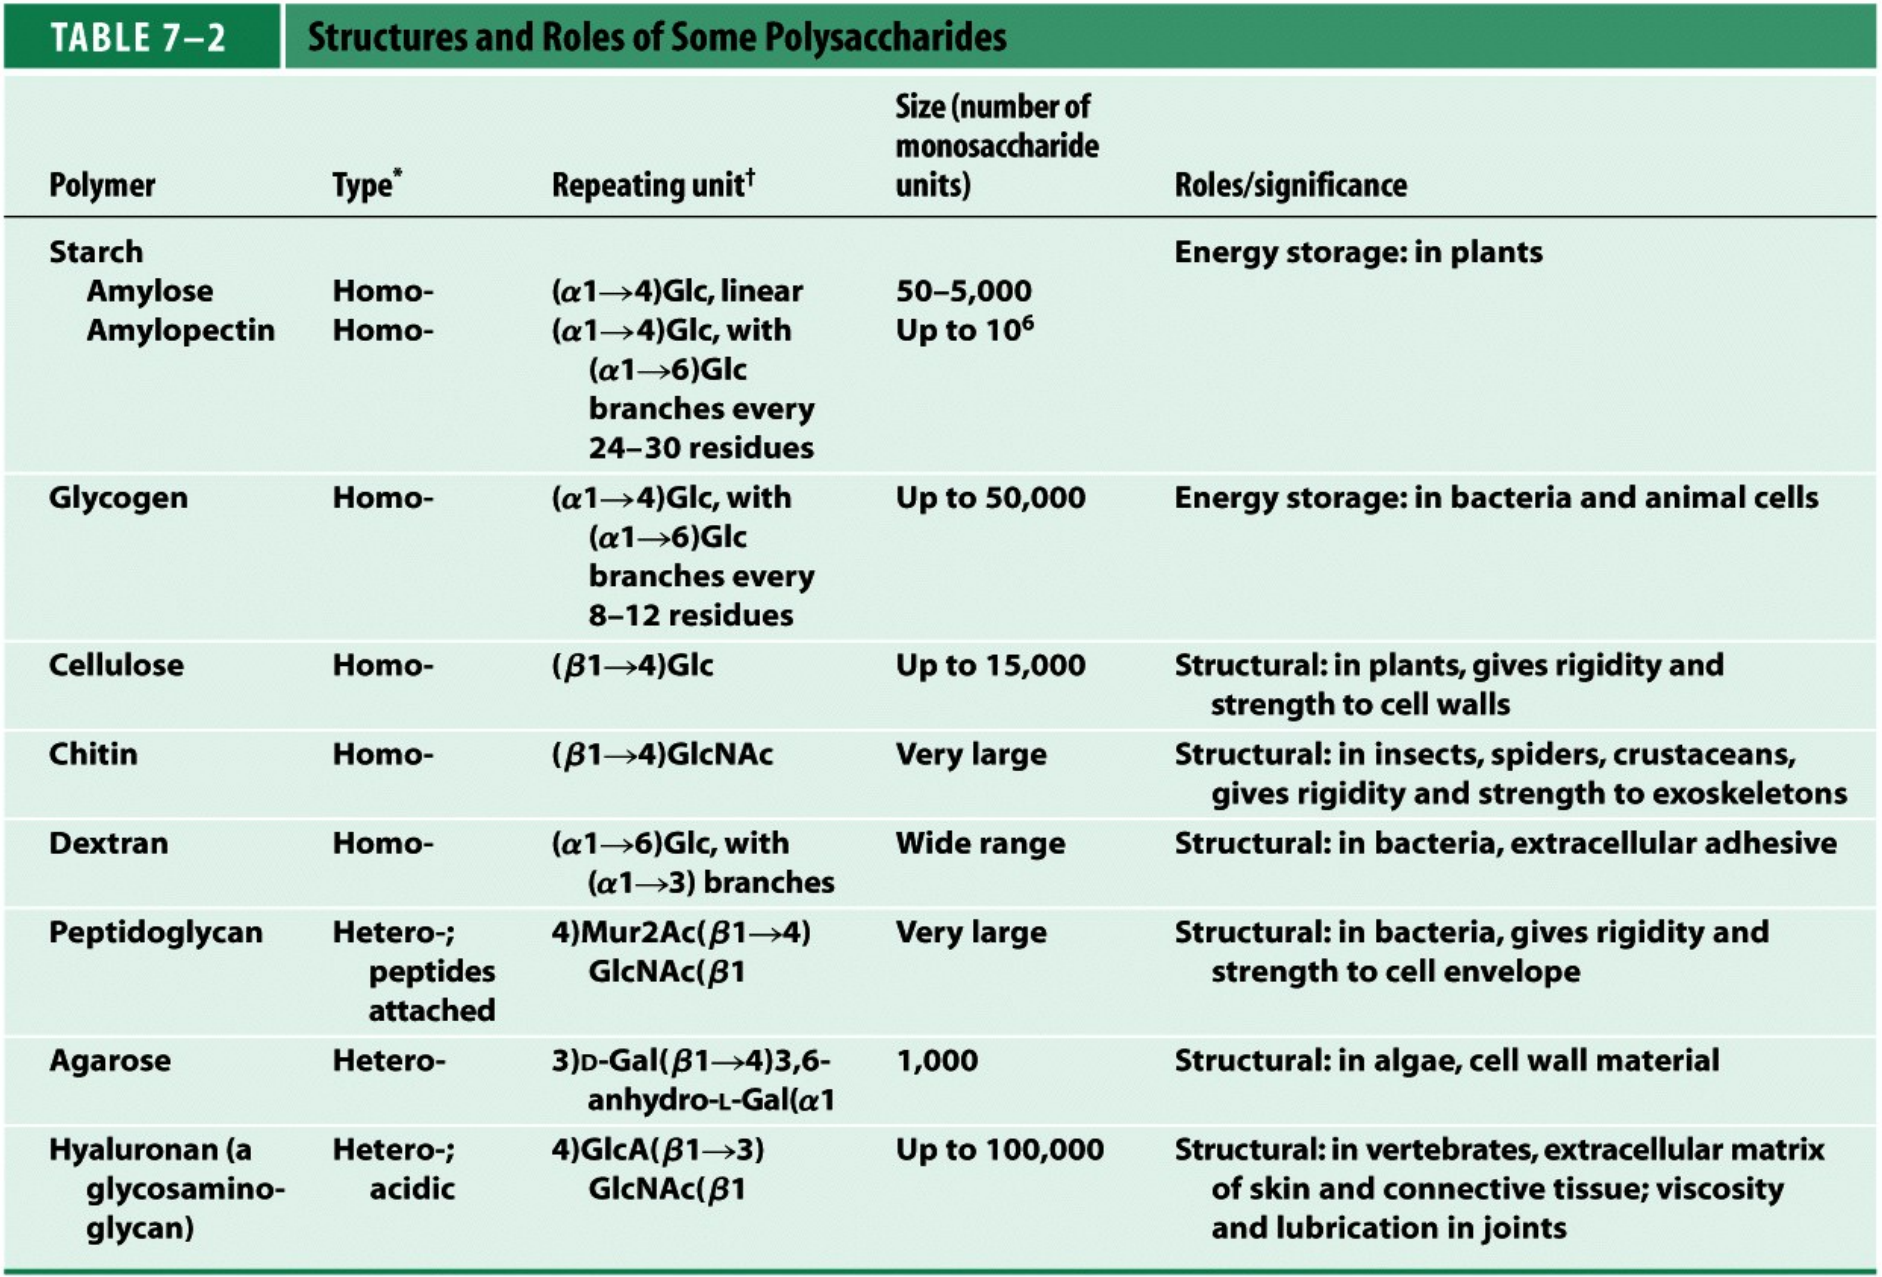
\includegraphics[width=\linewidth]{img/polysaccharide.png}
	\caption{Polysaccharide}
\end{figure}

\section{Nukleotide \& Nukleinsäuren}

\begin{description}
	\item[Nukleotide] Nukleobase + Pentose + Phosphat, Metabolismus (ATP, ADP), Cofaktoren (NAD+), Signalisierung (cAMP)
	\item[Nukleinsäuren] Genetische Informationen (DNA, RNA), Katalyse (Ribosome), Synthese (tRNA)
	\item[Phosphat-Gruppe] Bei neutralem pH negativ. Bei Nukleinsären an 5'
		Ende der Pentose. Mono-, Di-, Triphosphat je nach Anzahl
		Phosphat-Gruppen.
	\item[Pentose in Nukleotiden] $\beta$-D in RNA, $\beta$-2'-deoxy-D
		ribofuranose in DNA.
	\item[Nukleobasen] Derivate von Pyrmidin (Cytosin, Thymin, Uracil) oder
		Purin (Adenin, Guanin), absorbieren bei
		\SIrange{250}{270}{\nm}.
	\item[$\beta$-N-glycosidische Bindung] Verbindet Nukleobase mit
		Pentose, stabil gegen Hydrolyse, frei rotierbar.
	\item[Polynukleotide] Phosphodiester Bindung, negatives Rückgrat,
		stabil bei DNA, instabil bei RNA. 5' vs 3' Ende. Abbau bei RNA
		basenkatalisiert, Base deprotoniert Alkohol bei C2, \ce{O-}
		greift \ce{P} an, löst Phosphodiesterbindung.
	\item[siRNA] führt zur gezielten Zerschneidung gewisser mRNA,
		Abwehrmechanismus.
	\item[A-Form (RNA)] \SI{2.8}{\angstrom} pro Nukleotid, 11.5 Basen je
		Umdrehung, Basenpare geneigt zur Helixachse.
	\item[B-Form (DNA)] \SI{3.38}{\angstrom} pro Nukleotid, 10 Basen je
		Umdrehung, Basenpaare normal zur Helixachse.
	\item[RNA] >110 Basenpaarungen total, vielfältige Strukturen möglich.
	\item[Methylierung] Der Nukleobase zwecks Inaktivierung.
	\item[$T_m$ (melting point)] Hoher CG Gehalt (3 H Brücken), lange DNA,
		und hohe Salkzonzentration (Positive Ionen stabilisieren DNA)
		erhöhen Schmelzpunkt.
	\item[Sanger Methode] Replikation, wobei gewisser Anteil der Basen
		markiert ist, und so konstruiert dass Replikation abbricht.
		Danach Auftrennung der Fragmente in Gel, ablesen der Sequenz
		von unten nach oben.
	\item[Deaminierung] zB ca 100 C->U Mutationen je Tag und Säugerzelle.
		Base excision repair: Ersetzen aller U durch C in DNA.
	\item[Depurinierung] 10k Purin-Verluste je Tag und Säugerzelle.
	\item[Nucleotide excision repair] Falls durch UV Licht Bindung zwischen
		zwei benachbarten Basen (Dimer), Ausschnitt des ganzen Bereichs
		und Replikation.
\end{description}

\begin{figure}
	\centering
	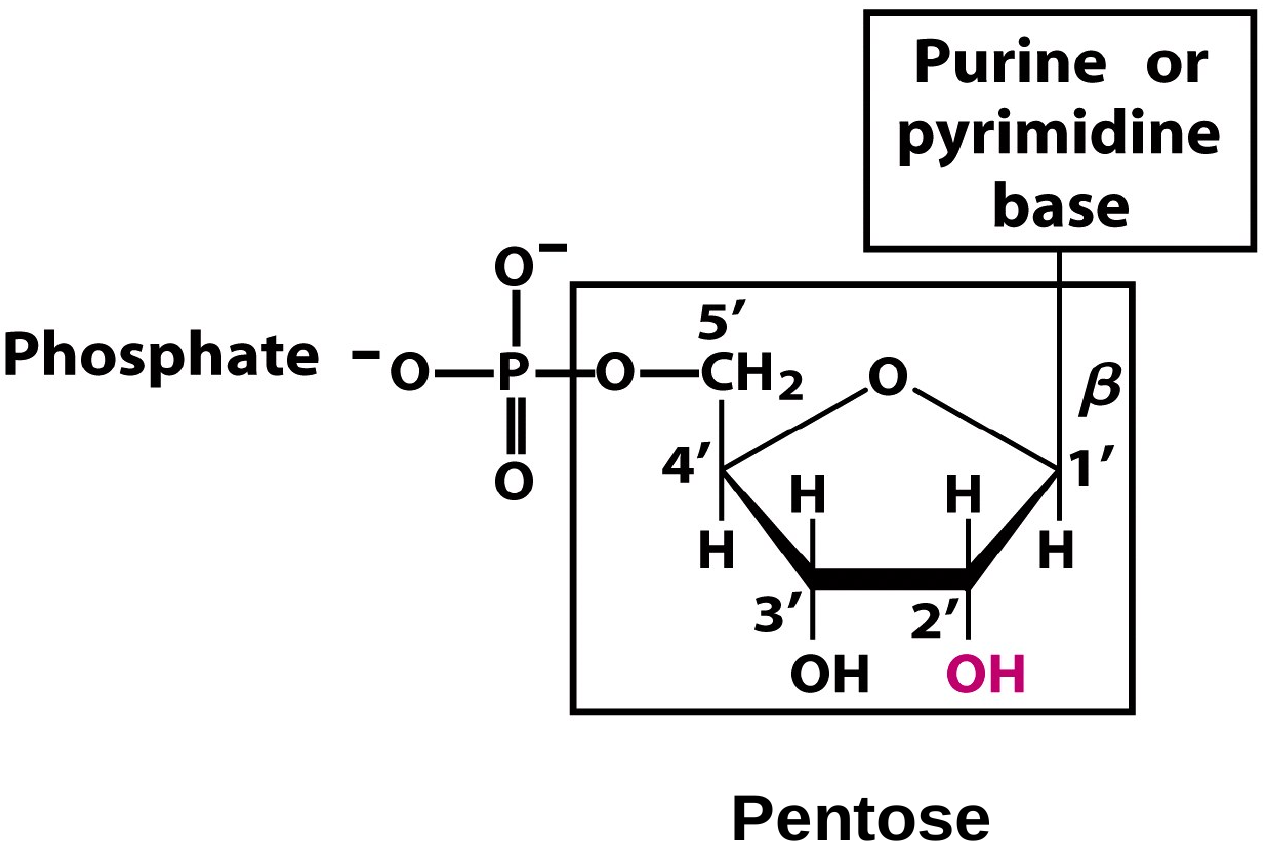
\includegraphics[width=\linewidth]{img/nukleotid.png}
	\caption{Nukleotid}
\end{figure}

\begin{figure}
	\centering
	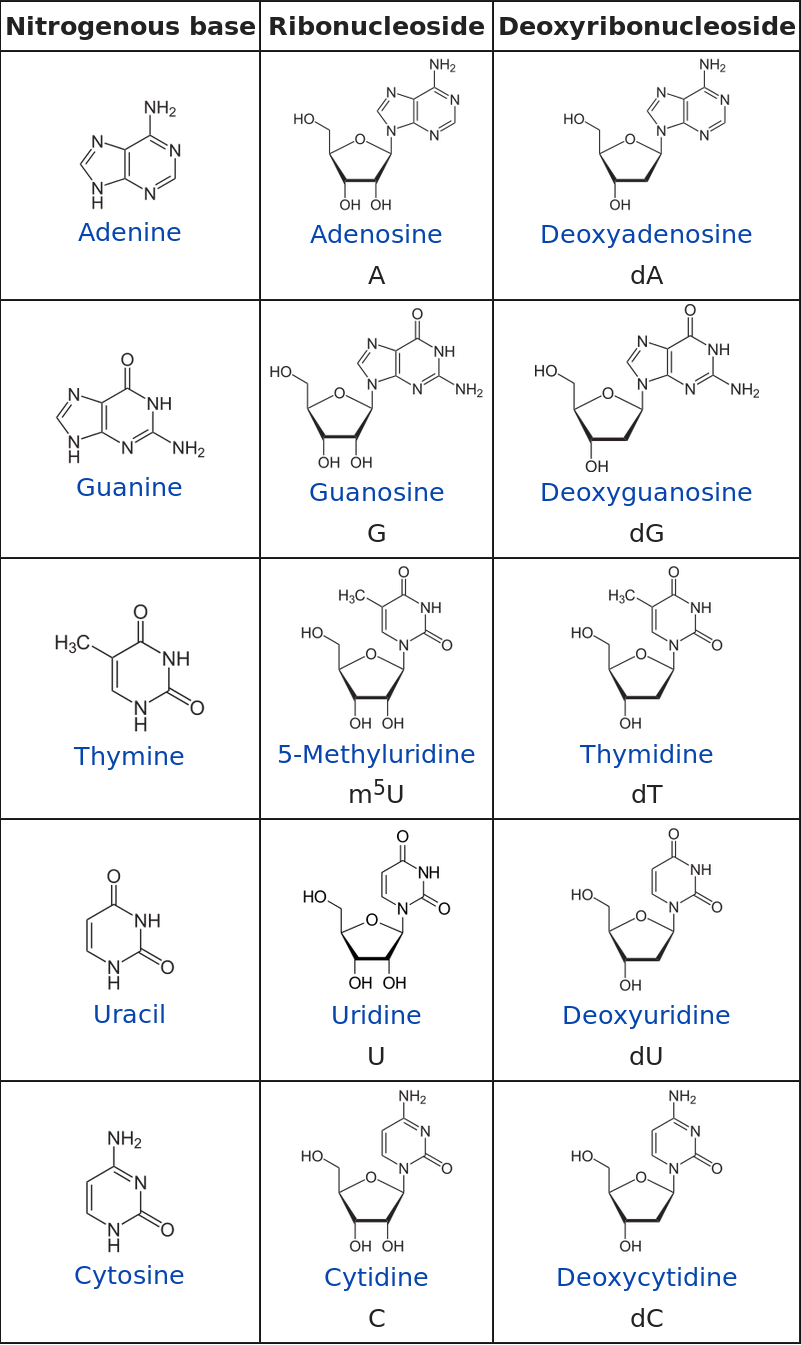
\includegraphics[width=\linewidth]{img/nukleoside.png}
	\caption{Nukleoside}
\end{figure}

\begin{figure}
	\centering
	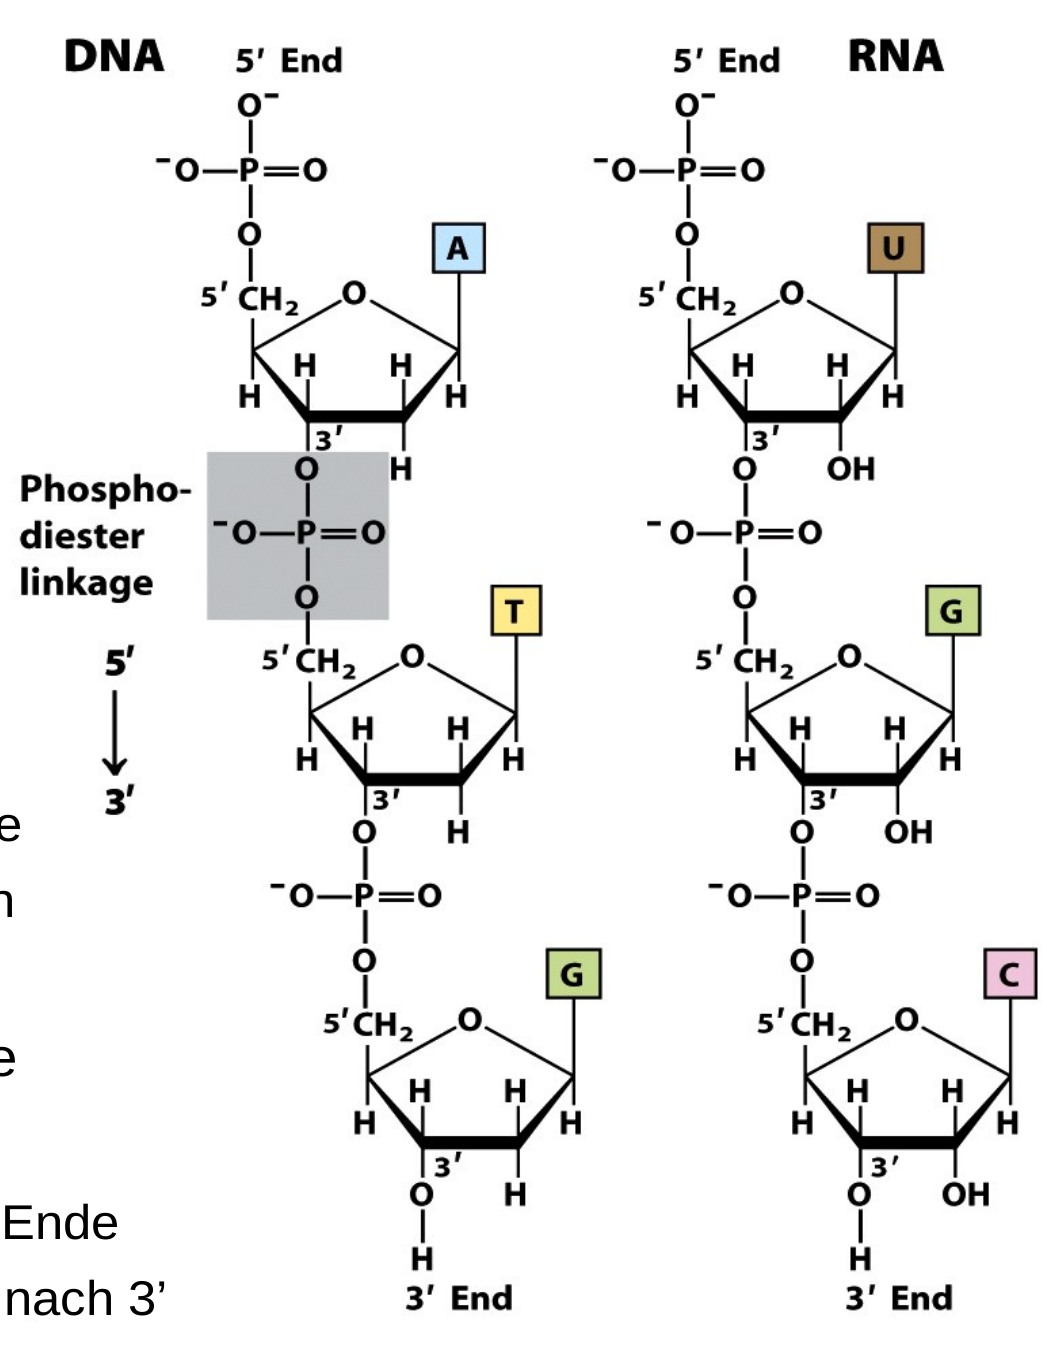
\includegraphics[width=\linewidth]{img/polynukleotide.png}
	\caption{Polynukleotide}
\end{figure}

\begin{figure}
	\centering
	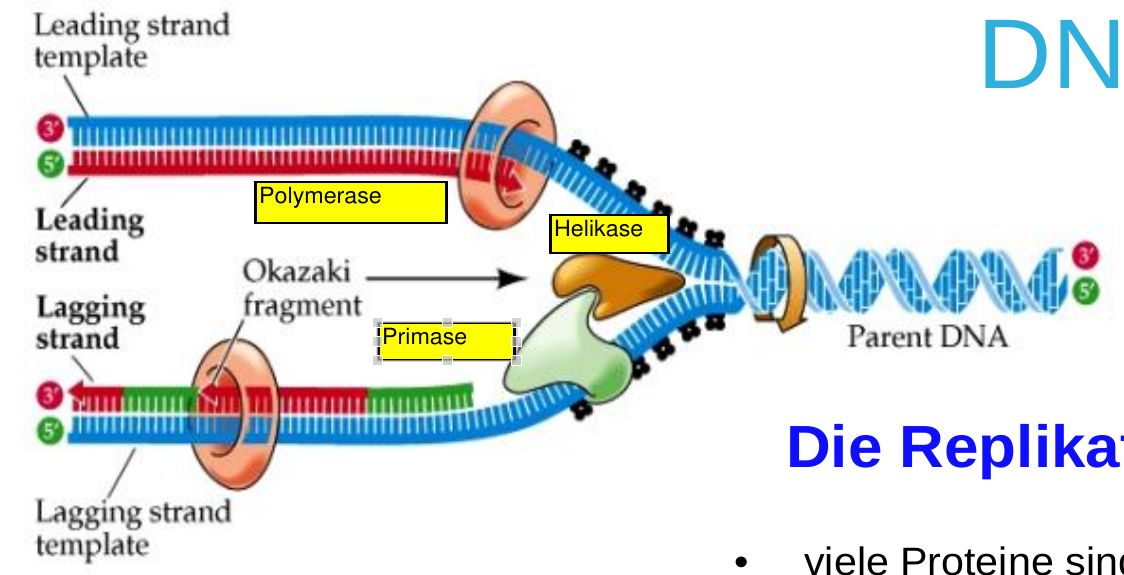
\includegraphics[width=\linewidth]{img/dna_replikation.png}
	\caption{DNA Replikation}
\end{figure}

\end{document}
